\section{第二次作业}

\begin{homework}[label={H:2-1}]
    Consider a unidirectional flow of incompressible fluid in a channel of width $2L$, driven by a constant pressure gradient $-\dv*{p}{x}$, with the fluid at rest at $t=0$. This unsteady flow $u(y, t)$ is governed by the following Navier-Stokes equation:
    \begin{equation}\label{E:2-1-1}
        \pdv{u}{t} = -\frac{1}{\rho}\dv{p}{x} + \nu\pdv[2]{u}{y},
        \quad
        -L\leq y\leq L,
    \end{equation}
    where $\nu$ is the fluid kinematic viscosity. Clearly, the initial and boundary conditions are
    \begin{equation}\label{E:2-1-2}
        u(x, t=0) = 0,
        \quad
        u(x=\pm L, t) = 0.
    \end{equation}

    \begin{enumerate}[label=(\alph*)]
        \item First, show that the steady state solution is given by
            \begin{equation}\label{E:2-1-3}
                u(y, t\to\infty) = u_0\qty(1-\frac{y^2}{L^2}),
            \end{equation}
            and determine the expression for $u_0$.
        \item Next, based on what we have obtained in class, write down the general time-dependent solution $u(y, t)$ analytically.
        \item What type (parabolic, hyperbolic, or elliptic) of partial differential equation is Equation~\eqref{E:2-1-1}?
    \end{enumerate}
\end{homework}

\paragraph{(a)}
由稳态(Steady state)可知 $\pdv*{u}{t}\equiv 0$,由压力梯度(Pressure gradient)恒定可将 $\dv*{p}{x}$ 视为常数。于是,可以将式~\eqref{E:2-1-3} 代入到式~\eqref{E:2-1-1} 中,整理后有
\begin{equation*}
    \frac{1}{\rho\nu}\dv{p}{x} = \pdv[2]{u}{y} = -\frac{2u_0}{L^2}
    \quad
    \text{where } u=u(y, t\to\infty),
\end{equation*}
即
\begin{equation*}
    u_0 = -\frac{L^2}{2\rho\nu}\dv{p}{x}.
\end{equation*}

\paragraph{(b)}
由课堂上的推导,可知偏微分方程的解析解为
\begin{equation*}
    \begin{aligned}
        \frac{u(y, t)}{u_0} &= f\qty(\frac{y}{L}, \frac{\nu t}{L^2}) \\
                            &= \qty(1 - \frac{y^2}{L^2}) - \sum_{k=0}^\infty\frac{4(-1)^k}{\qty[\pi(k+0.5)]^3}\exp\qty[-\frac{(k+0.5)^2\pi^2\nu t}{L^2}]\cos\qty[(k+0.5)\pi\frac{y}{L}],
    \end{aligned}
\end{equation*}
即
\begin{equation*}
    u(y, t) = -\frac{L^2}{2\rho\nu}\dv{p}{x} \qty{
        \qty(1 - \frac{y^2}{L^2}) - \sum_{k=0}^\infty\frac{4(-1)^k}{\qty[\pi(k+0.5)]^3}\exp\qty[-\frac{(k+0.5)^2\pi^2\nu t}{L^2}]\cos\qty[(k+0.5)\pi\frac{y}{L}]
    }.
\end{equation*}

\paragraph{(c)}
式~\eqref{E:2-1-1} 在空间与时间上均为抛物型(Parabolic)偏微分方程。



\begin{homework}[label={H:2-2}]
    We now solve the last problem numerically, by the following algorithm: the explicit Euler scheme in time, and central finite-difference in space,
    \begin{equation}\label{E:2-2-1}
        \frac{u^{n+1}_j-u^n_j}{\Delta t}
        =
        -\frac{1}{\rho}\dv{p}{x} + \nu\frac{u^n_{j-1}-2u^n_j+u^n_{j+1}}{\Delta y^2},
    \end{equation}
    where $\Delta y=2L/N$, $u^n_j=u(y_j, t_n)$ with $y_j=-L+(j-1)\Delta y$ and $t_n=n\Delta t$ ($n=0, 1, 2, 3, \ldots$). The two end nodes $j=1$ and $j=N+1$ are located on the channel walls. Assume $L=1$, $u_0=1$, and $\nu=0.1$. The time step size will be set according to $\Delta t=0.32\Delta y^2/\nu$.

    \begin{enumerate}[label=(\alph*)]
        \item Start with the code Dr.\ Wang provided in Lecture 1. Run the code with $N=8, 16, 32$.  Plot and compare the velocity profiles from different grid resolutions at $\nu t/L^2=1.28m/N^2=0.2, 1.0, 10.0$, where $m$ is the number of time steps. You need to modify Dr. Wang's code as needed. You also need to find a nice plotting package (e.g. UCAR's NCL) to do the plots. Also find out at what dimensionless time, $\nu t/L^2$, the velocity at the center of the channel ($y=0$) reaches the value of $0.99u_0$ (meaning the steady state is essentially reached) for the three different grid resolutions, respectively.
        \item Use the analytical solution as the benchmark, plot the errors at $\nu t/L^2=0.2, 1.0, 10.0$, for the three grid resolutions in~(a). Make your own observations.
        \item Plot and compare the time evolution of the properly normalized wall viscous stress from the three resolutions and the analytical solution. Explain how to compute the wall viscous stress for both the numerical and analytical solutions.
        \item Summarize any problems you have encountered when doing this problem, and what you have learned after doing this problem (in numerical method, coding, plotting, accessing the department Unix server, Unix system, etc.).
    \end{enumerate}
\end{homework}

根据 Homework~\ref{H:2-2},可以编写如附录~\ref{S:appendix-fortran} 中 Code~\ref{C:2-2-1} 与 Code~\ref{C:2-2-2} 所示的偏微分方程数值求解的代码。此外,本文选择 \href{https://github.com/matplotlib/matplotlib}{matplotlib} 作为可视化工具,可以编写如附录~\ref{S:appendix-python} 中 Code~\ref{C:python-unidirectional_flow} 所示的可视化代码。

\paragraph{(a)}
不同网格数量($N$)与无量纲时间(Dimensionless time,$\nu t/L^2$)下速度的数值解如表~\ref{T:2-2-1} 所示。当固定无量纲时间为 1.0 时,不同网格数量下的速度如图~\ref{F:2-2-1} 所示;当固定网格数量为 32 时,不同无量纲时间下的速度如图~\ref{F:2-2-2} 所示。

\begin{figure}[H]
    \centering
    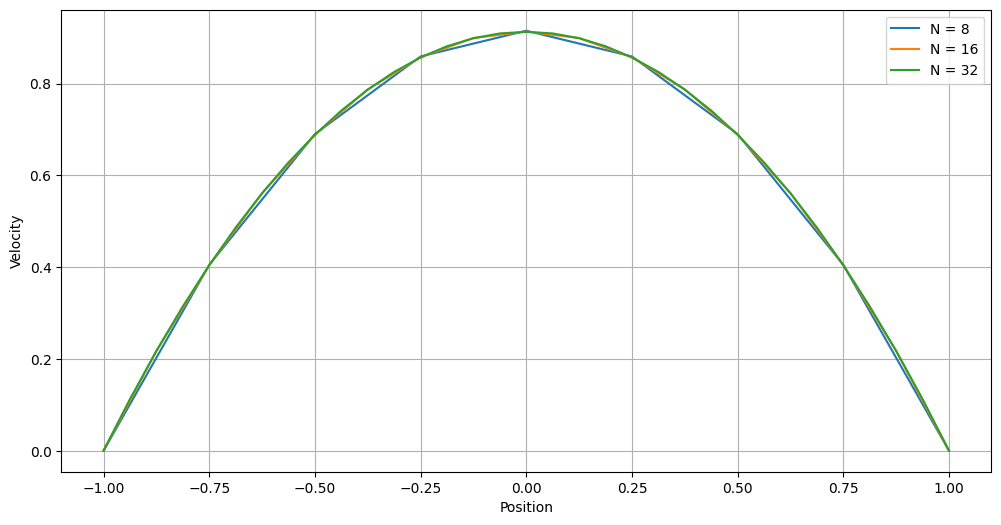
\includegraphics[width=.75\textwidth]{figure/2/grid.png}
    \caption{固定无量纲时间,改变网格数目}\label{F:2-2-1}
\end{figure}

\begin{figure}[H]
    \centering
    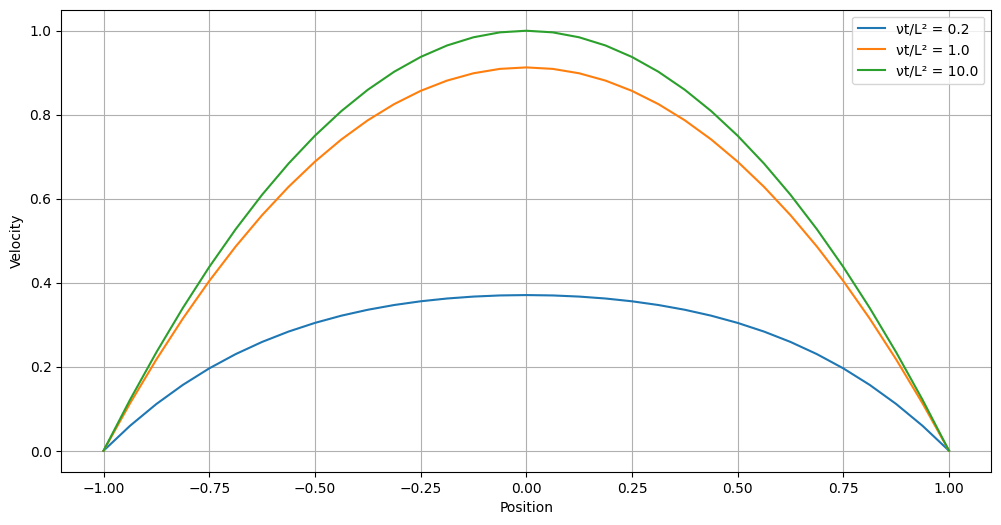
\includegraphics[width=.75\textwidth]{figure/2/velocity.png}
    \caption{固定网格数目,改变无量纲时间}\label{F:2-2-2}
\end{figure}

当 $\Delta t=0.32\Delta y^2/\nu$ 时,要想在最后的时间步下通道(Channel)中心的速度达到 $0.99u_0$,需要通过不断增加时间步的方式来找寻临界点,最后,再反推出无量纲时间。通过实验可以发现,达到要求的无量纲时间的取值会随着网格数量的变化而变化:当网格数量为 8 时,时间步为 93,无量纲时间为 \num{1.860000};当网格数量为 16 时,时间步为 375,无量纲时间为 \num{1.875000};当网格数量为 32 时,时间步为 1503,无量纲时间为 \num{1.878750}。本文为找寻在题目给定的时间步长下无量纲时间随网格数量增加的大致趋势,分别将网格数量设置为从 2 到 128 的偶数,并相应地计算出达到要求的无量纲时间,可以得到如图~\ref{F:2-2-3} 所示的趋势图。根据趋势图可以大概猜测出,无量纲时间会随着网格数量的增加而逐步趋近于某个特定的值。

\begin{figure}[H]
    \centering
    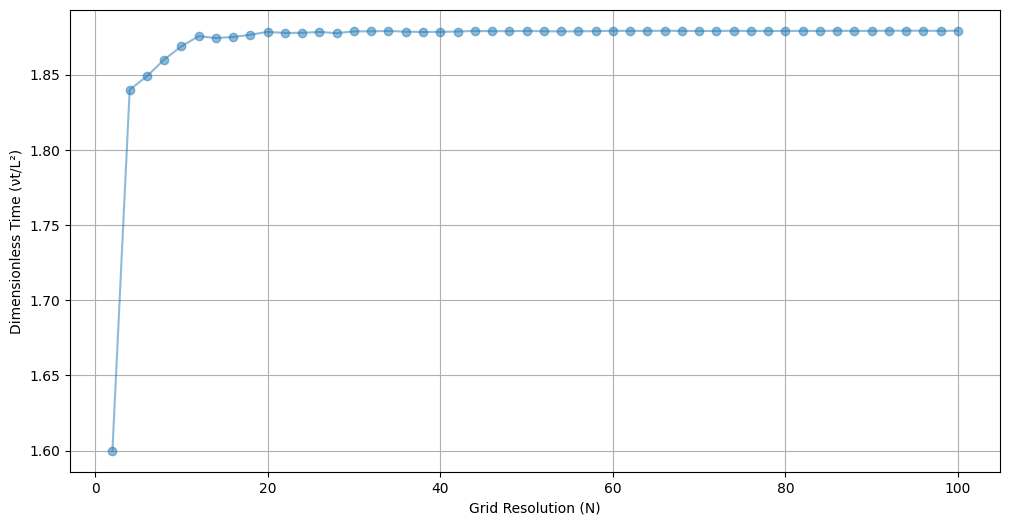
\includegraphics[width=.75\textwidth]{figure/2/dimensionless_time.png}
    \caption{无量纲时间随网格数量增加的趋势图}\label{F:2-2-3}
\end{figure}

\paragraph{(b)}
在不同无量纲时间下速度的数值解与解析解之间的误差如表~\ref{T:2-2-1} 所示,可以大概观测出越远离边缘误差越大,同时随着网格数量与无量纲时间的增加,速度的数值解与解析解之间的误差减少。如果将速度的数值解与解析解分别记为 $u_{\mathrm{n}}$ 与 $u_{\mathrm{a}}$,则可绘制如图~\ref{F:2-2-2} 所示的 $\log_{10}\norm{u_{\mathrm{n}}-u_{\mathrm{a}}}_2$ 的等高线图,可以看出速度的数值解与解析解之间的误差并不总是随着网格数量与无量纲时间的增加而减少。

\begin{figure}[H]
    \centering
    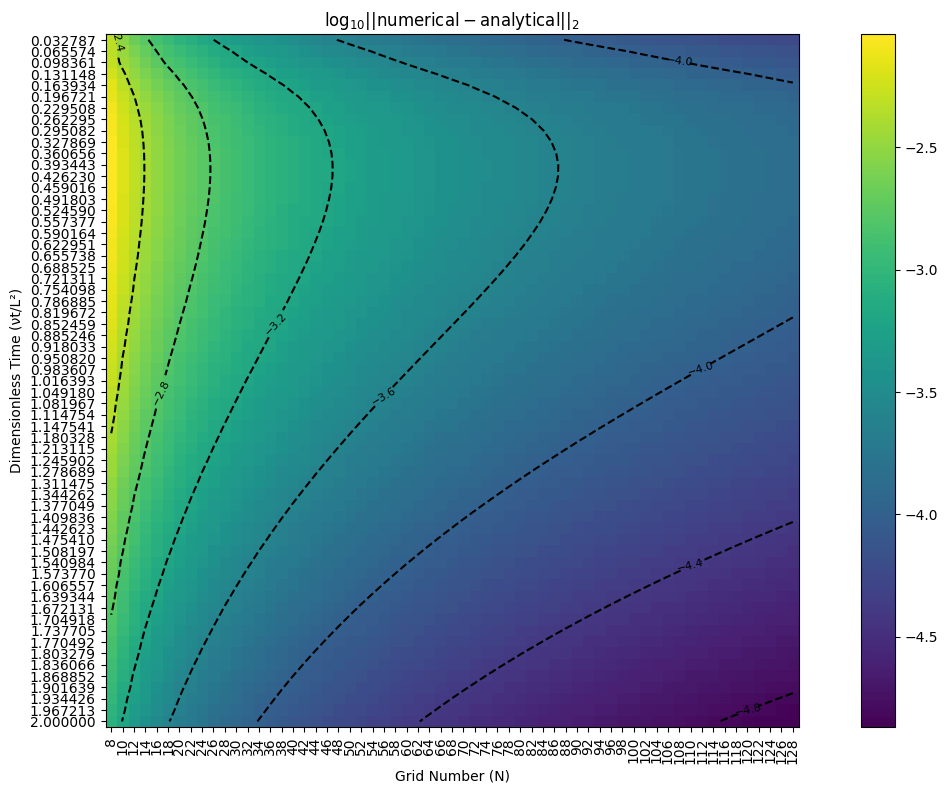
\includegraphics[width=.8\textwidth]{figure/2/error.png}
    \caption{$\log_{10}\norm{u_{\mathrm{n}}-u_{\mathrm{a}}}_2$ 等高线图}\label{F:2-2-2}
\end{figure}

\begin{landscape}
    \begin{table}[h]
        \renewcommand{\arraystretch}{3}
        \centering
        \caption{不同网格数量与无量纲时间下速度的数值解、解析解及其误差}\label{T:2-2-1}
        \begin{tabular}{c|ccc}
            $\nu t/L^2$ &                                                        $N=8$ &                                                        $N=16$ &                                                        $N=32$ \\ \hline
                    0.2 &  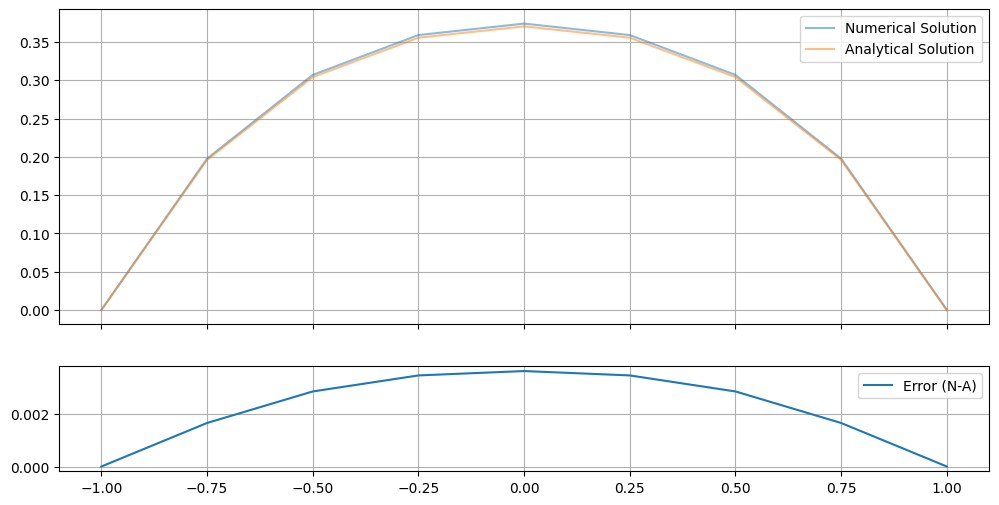
\includegraphics[height=0.23\textwidth]{figure/2/8-0.2.png} &  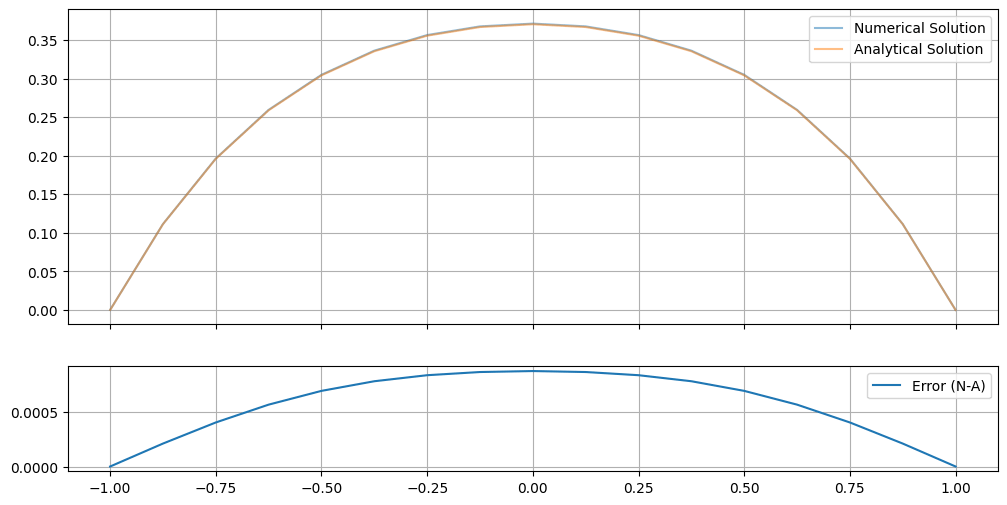
\includegraphics[height=0.23\textwidth]{figure/2/16-0.2.png} &  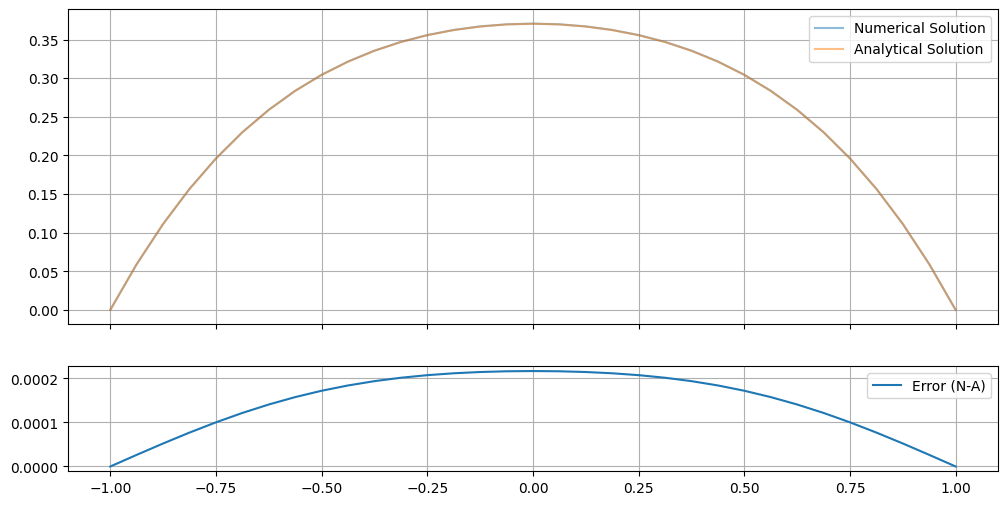
\includegraphics[height=0.23\textwidth]{figure/2/32-0.2.png} \\
                    1.0 &  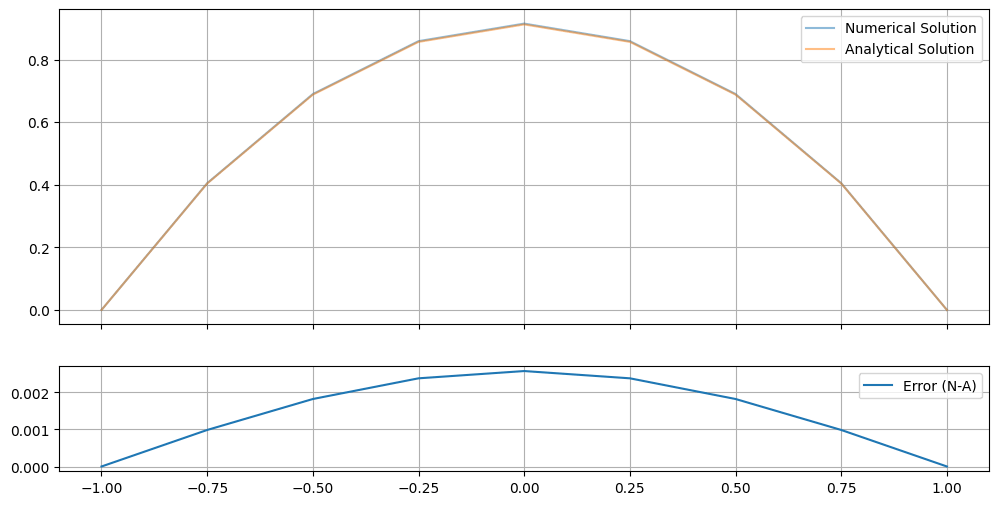
\includegraphics[height=0.23\textwidth]{figure/2/8-1.0.png} &  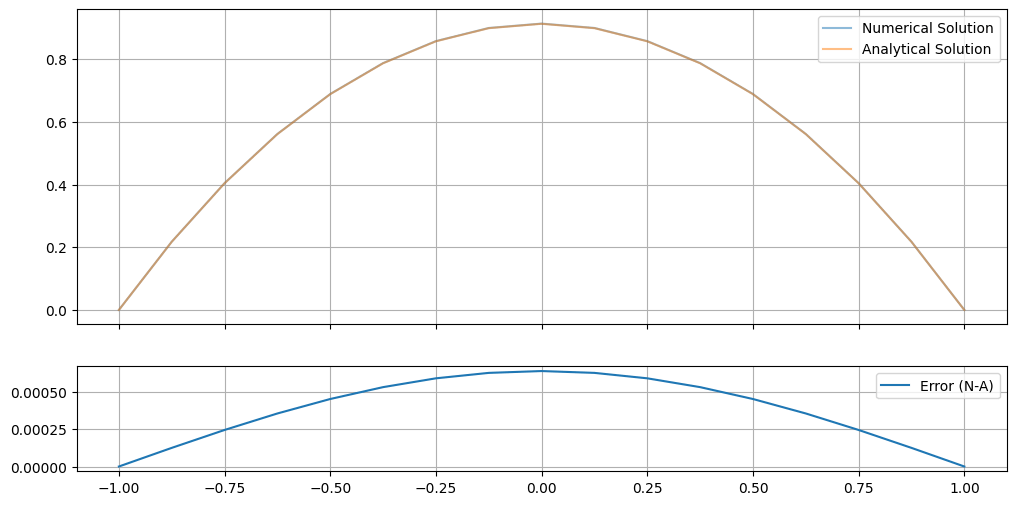
\includegraphics[height=0.23\textwidth]{figure/2/16-1.0.png} &  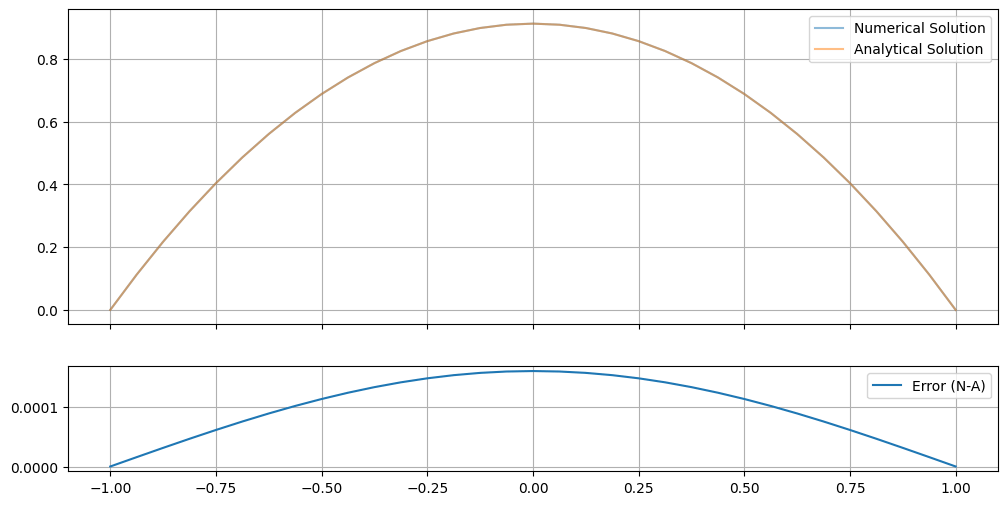
\includegraphics[height=0.23\textwidth]{figure/2/32-1.0.png} \\
                   10.0 & 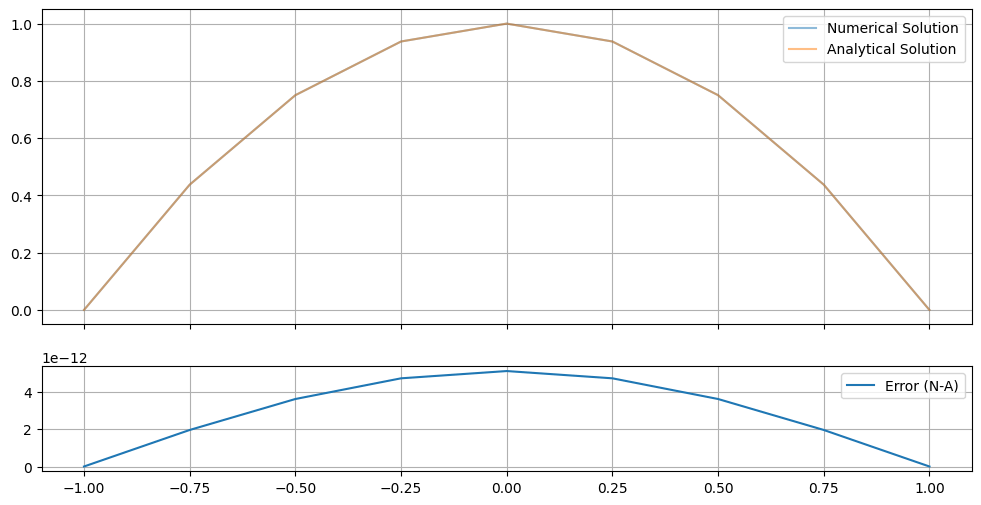
\includegraphics[height=0.23\textwidth]{figure/2/8-10.0.png} & 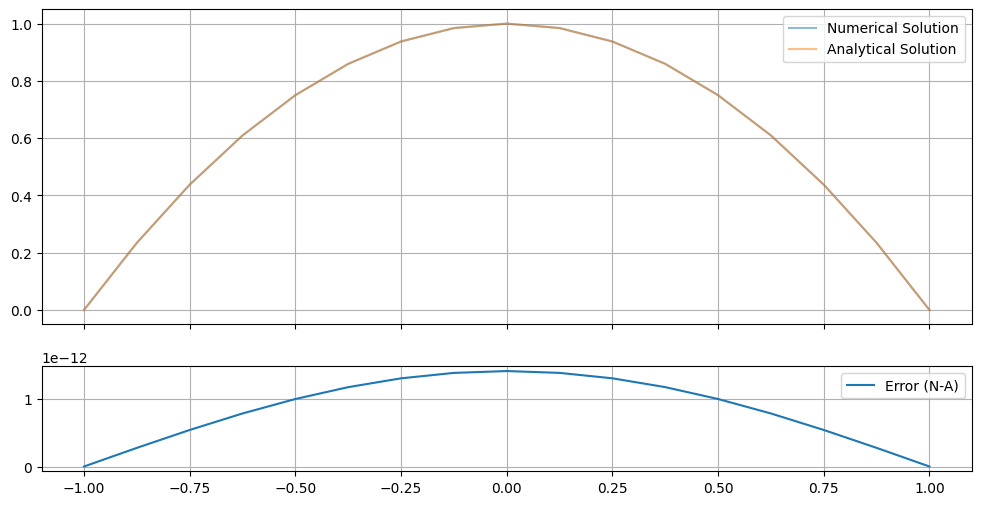
\includegraphics[height=0.23\textwidth]{figure/2/16-10.0.png} & 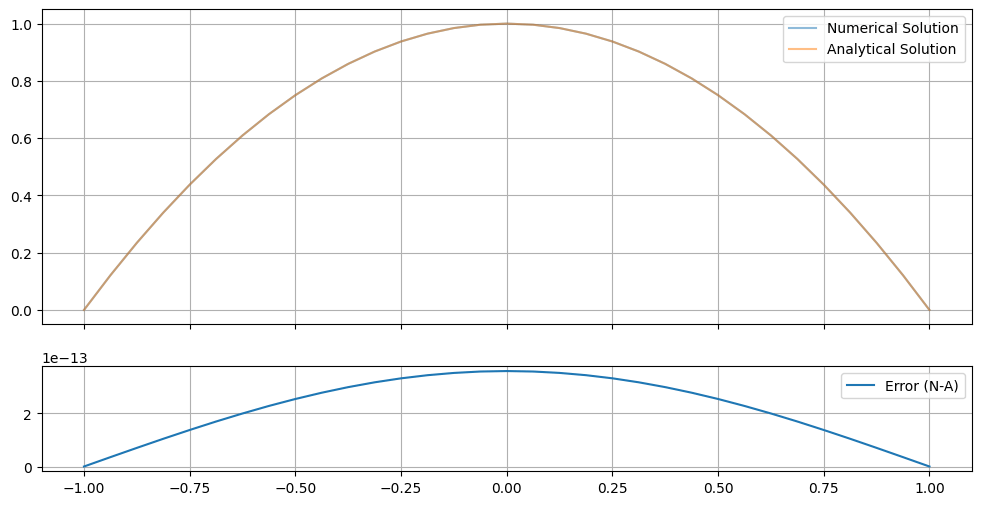
\includegraphics[height=0.23\textwidth]{figure/2/32-10.0.png}
        \end{tabular}
    \end{table}
\end{landscape}

\paragraph{(c)}
壁面粘性应力(Wall viscous stress)的计算公式为 $\tau_w=\mu\qty(\pdv*{u}{y})_{y=\pm L}=\rho\nu\qty(\pdv*{u}{y})_{y=\pm L}$,数值解是需要通过数值差分计算,而解析解则是直接求偏导数即可。前面的系数题目中没有给出,所以标准化(Normalized)可能是指去掉前面的系数,因此计算公式变为 $\tau^*_w=\qty(\pdv*{u}{y})_{y=\pm L}$。如图~\ref{F:2-2-4} 为 $y=-L$ 处标准化壁面粘性应力在不同网格数量下随无量纲时间的趋势图,其中蓝线为标准化壁面粘性应力的解析解,可以大概观测出,随着网格数量的增加,数值解将不断逼近解析解。因为算例对称,$y=L$ 处的标准化壁面粘性应力与 $y=-L$ 处的方向相反,结果互为相反数。

\begin{figure}[H]
    \centering
    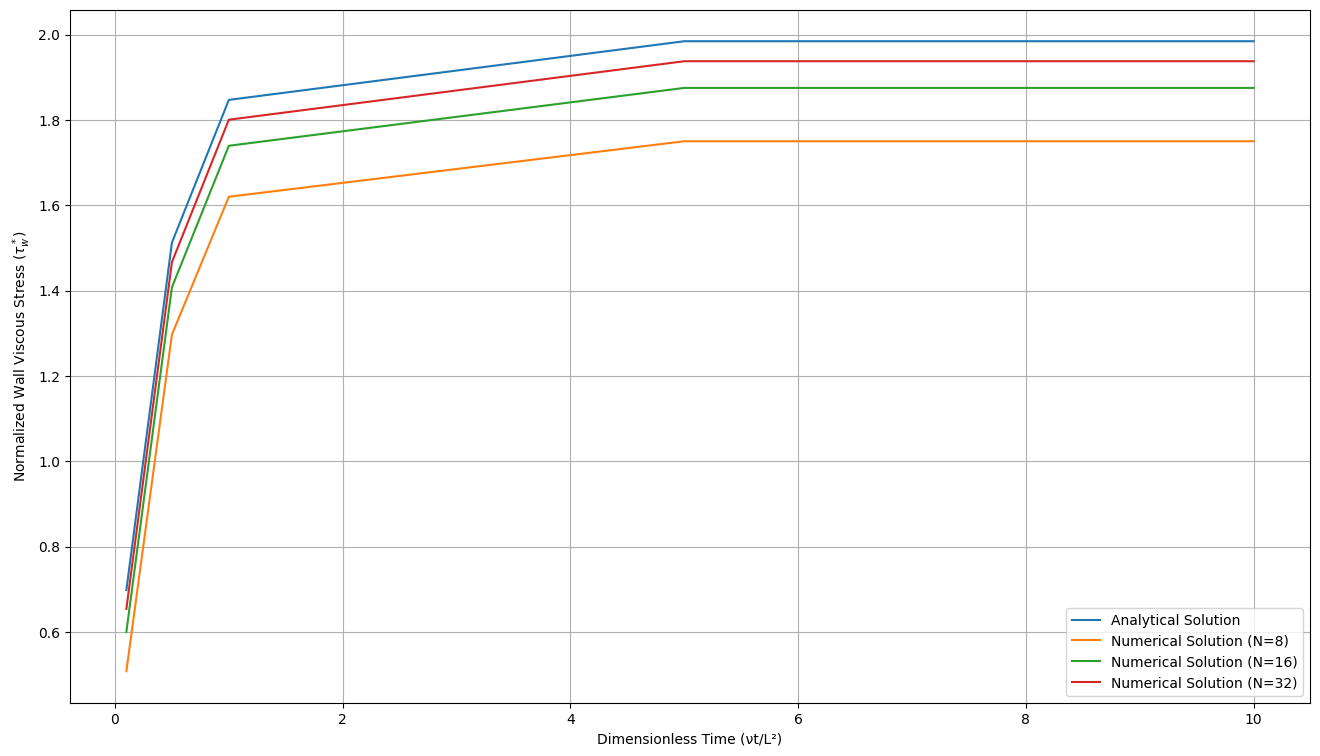
\includegraphics[width=.75\textwidth]{figure/2/normalized_wall_viscous_stress.png}
    \caption{标准化壁面粘性应力的数值解与解析解}\label{F:2-2-4}
\end{figure}

\paragraph{(d)}
\texttt{Fortran} 的 \texttt{function} 与 \texttt{subroutine} 不同于其他编程语言,需要针对场合使用不同的实现。



\begin{homework}[label={H:2-3}]
    The basic fluid mechanics equations contain the continuity, momentum, and energy equations as follows:
    \begin{subequations}\label{E:2-3-1}
        \begin{align}
            \pdv{\rho}{t} + \pdv{(\rho u_j)}{x_j} &= 0 \label{E:2-3-1-a} \\
            \rho\pdv{u_i}{t} + \rho u_j\pdv{u_i}{x_j} &= \rho g_i + \pdv{\tau_{ij}}{x_j} \label{E:2-3-1-b} \\
            \rho\pdv{e}{t} + \rho u_j\pdv{e}{x_j} &= -p\pdv{u_j}{x_j} + \rho\varepsilon - \pdv{q_j}{x_j} \label{E:2-3-1-c}
        \end{align}
    \end{subequations}
    where the total stress tensor and the heat flux are given as
    \begin{equation}\label{E:2-3-2}
        \tau_{ij} = \qty(-p + \mu^V\pdv{u_k}{x_k}\delta_{ij}) + 2\mu\qty(S_{ij} - \frac{1}{D}\pdv{u_k}{x_k}\delta_{ij}),
        \quad
        q_j = -k\pdv{T}{x_j}
    \end{equation}
    where $D$ is the number of space dimensions ($D=2$ or $D=3$). The rate of viscous dissipation is
    \begin{equation}\label{E:2-3-3}
        \rho\varepsilon = 2\mu\qty(S_{ij} - \frac{1}{D}\pdv{u_k}{x_k}\delta_{ij})^2 + \mu^V\qty(\pdv{u_k}{x_k})^2
    \end{equation}
    where $\mu$ and $\mu^V$ are shear and bulk viscosity, respectively. The strain rate is $S_{ij}\equiv\frac{1}{2}\qty(\pdv{u_i}{x_j}+\pdv{u_j}{x_i})$.

    \begin{enumerate}[label=(\alph*)]
        \item What specific physical law does each of Equations~\eqref{E:2-3-1}, represent?
        \item What are the physical meanings of $\tau_{ij}$ and $q_j$?
        \item What is the physical significance of the quantity $\varepsilon$?
        \item List the physical dimensions of all quantities involved in the above equations.
    \end{enumerate}
\end{homework}

\paragraph{(a)}
式~\eqref{E:2-3-1-a} 对应质量守恒(连续性方程),式~\eqref{E:2-3-1-b} 对应动量守恒(动量方程),式~\eqref{E:2-3-1-c} 对应能量守恒(能量方程方程)。

\paragraph{(b)}
$\tau_{ij}$ 意味着单位面积的粘性力;$q_j$ 意味着单位体积沿 $x$ 方向传导的能量。

\paragraph{(c)}
$\varepsilon$ 的物理意义为由粘性产生的热量。

\paragraph{(d)}

\begin{center}
    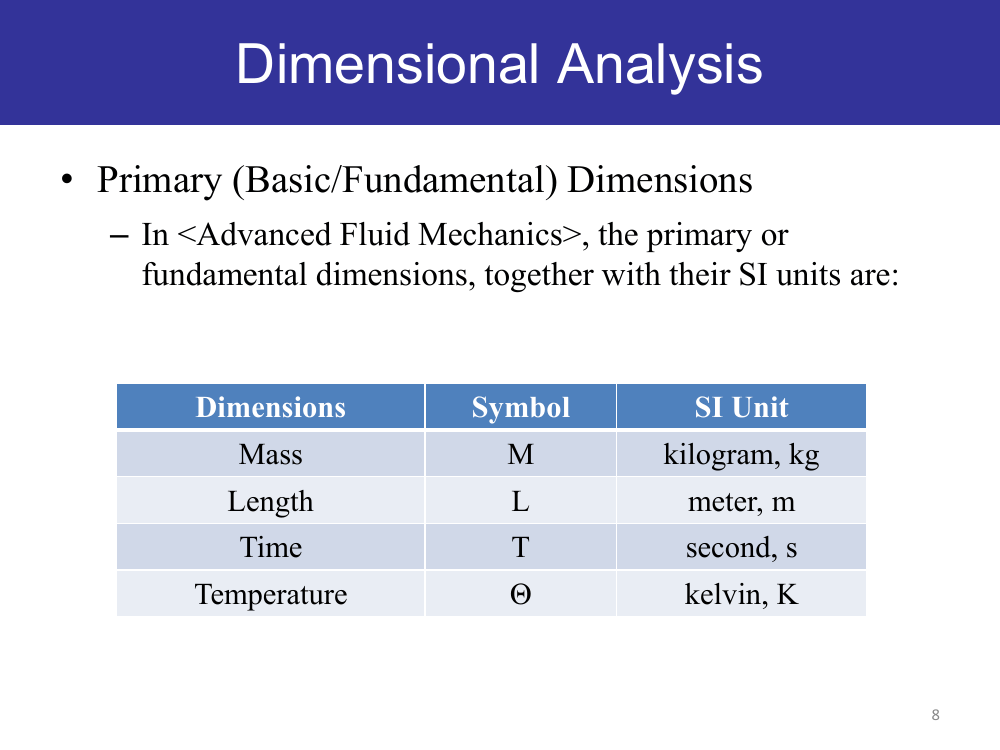
\includegraphics[width=.65\textwidth]{figure/2/dimensional_analysis/1.png}

    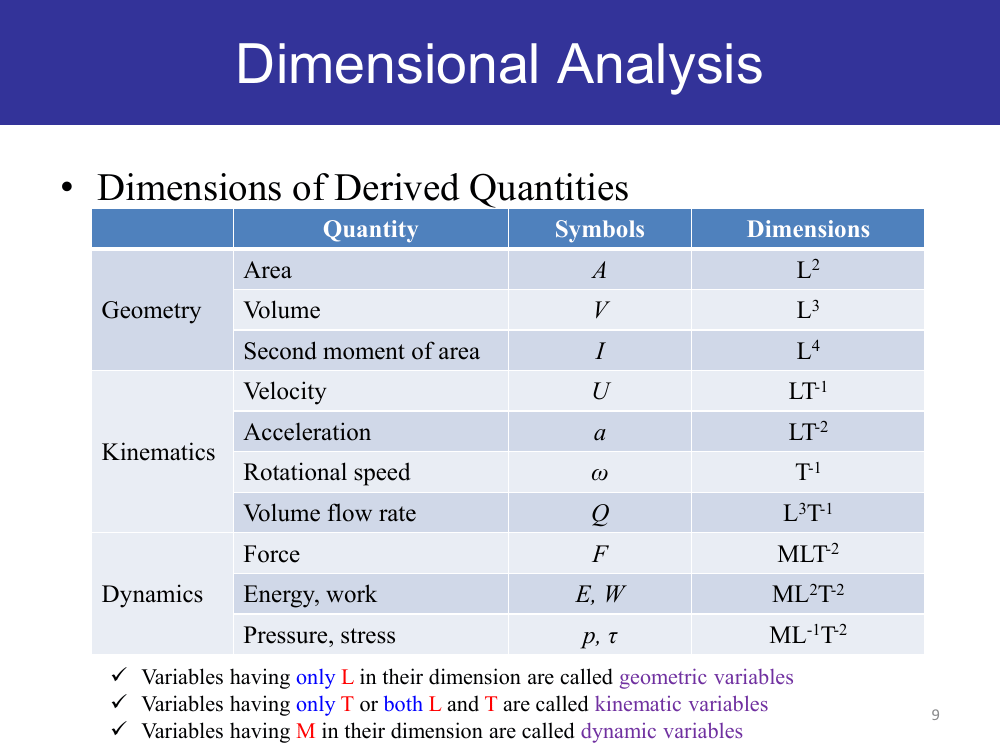
\includegraphics[width=.65\textwidth]{figure/2/dimensional_analysis/2.png}

    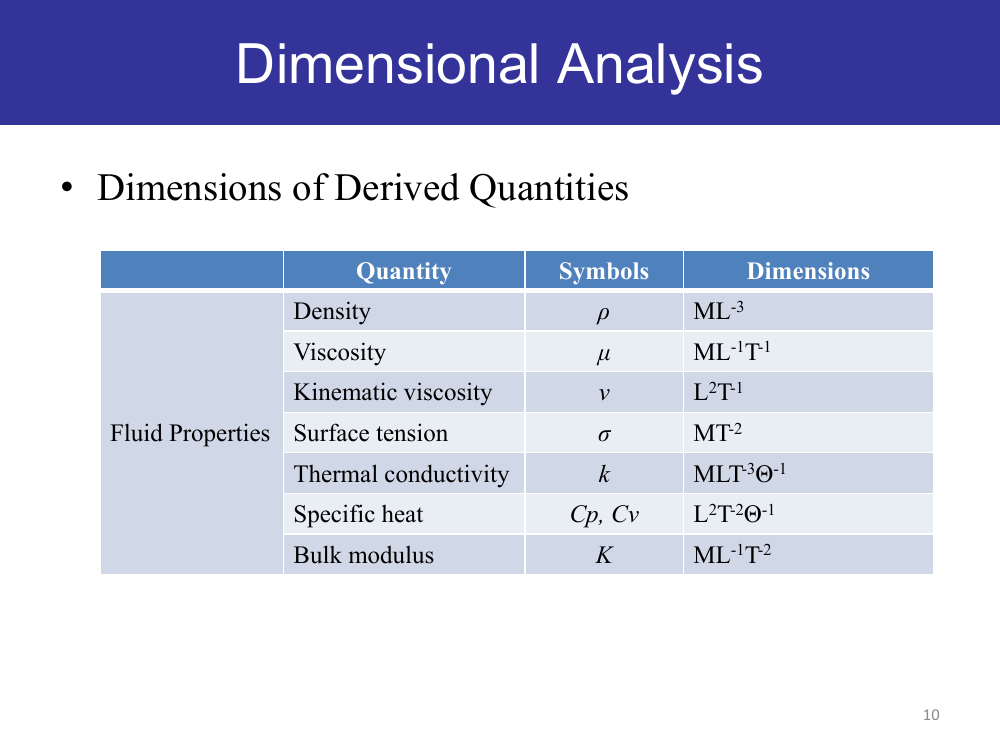
\includegraphics[width=.65\textwidth]{figure/2/dimensional_analysis/3.png}
\end{center}



\begin{homework}[label={H:2-4}]
    In the class, we discuss the flux Jacobian for the 1D linearized, isentropic acoustic wave equations
    \begin{equation}\label{E:2-4-1}
        \pdv{F(U)}{U} = \mqty(0 & \rho_0 \\ c^2_s/\rho_0 & 0)
    \end{equation}
    where $\rho_0$ is the base (background) density and $c_s\equiv\sqrt{\gamma p/\rho}$ is the speed of the sound.

    \begin{enumerate}[label=(\alph*)]
        \item Determine the eigenvalues and corresponding eigenvectors for the matrix;
        \item Based on the results in part~(a), work out the diagonal decomposition of the matrix as $R\Lambda R^{-1}$.
    \end{enumerate}
\end{homework}

\paragraph{(a)}
矩阵的特征值为 $\pm c_s$,对应的特征向量为 $\mqty(\rho_0 & \pm c_s)^T$。

\paragraph{(b)}
如式~\eqref{E:2-4-2} 所示。

\begin{equation}\label{E:2-4-2}
    \pdv{F(U)}{U} =
        \mqty(\rho_0 & \rho_0 \\ c_s & -c_s)
        \mqty(c_s & \\ & -c_s)
        \mqty(-\frac{1}{2\rho_0} & \frac{1}{2\c_s} \\ \frac{1}{2\rho_0} & -\frac{1}{2c_s}).
\end{equation}
